
\documentclass[oneside]{um-fict}

\usepackage{verbatim}
\usepackage{amsfonts}
\usepackage{amsmath}
\usepackage{amssymb}
\usepackage{amsthm}
\usepackage{pdfpages}
\usepackage{amssymb}
\usepackage{graphicx}
\usepackage{listings}
\usepackage{proof}
\usepackage{xcolor}
\usepackage{titlesec}
\usepackage{rotating}
\usepackage{float}
\usepackage{tikz}
\usepackage{url}
\usepackage{xurl}

\definecolor{OliveGreen}{rgb}{0,0.6,0}


\lstset{
  language=C,
  frame=tb,
  aboveskip=3mm,
  basicstyle=\footnotesize\ttfamily,
  numbers=left,
  stepnumber=1,
  numbersep=10pt,
  tabsize=4,
  columns=flexible,
  numbers=none,
  numberstyle=\tiny\color{gray},
  keywordstyle=\color{blue},
  commentstyle = \color{OliveGreen},
  stringstyle=\color{purple},
  breaklines=true,
  breakatwhitespace=true,
  showstringspaces=false,
  tabsize=3,
  numbers=left
}

\title{JavaScript Framework for Actor-Based Programming}
\author{Andrew Buhagiar}            
\authorID{373801L}                  
\supervisor{Prof Kevin Vella}      

\degreeName{B.Sc. I.C.T. (Hons.)}                                       
\doctype{dissertation}               
\degreeDate{\monthyeardate\today}    
\graphicspath{{./images/}{./chap1/images/}{./chap2/images/}}

\makeindex


\begin{document}
\frontmatter 
\maketitle
\begin{acknowledgements}
I thank Prof.\ Kevin Vella for his continuous support, patience, and advice which allowed me to complete the objectives of this project.

I also extend my gratitude to my family for their investment which allowed me to pursue my studies.
\end{acknowledgements}
\begin{abstract}
\hspace{5mm}This dissertation explores the suitability of the actor model when used to bring concurrency and parallelism to JavaScript. Actors are concurrent isolated units of computation which process messages using their predefined behaviour. The implementation takes the form of two APIs for both the Node.js and browser environments respectively, allowing developers to intuitively reason about engineering JavaScript programs through the spawning and sending of messages to actors.

\hspace{5mm}Isolated actors can be safely spawned on remote devices over a network as well as utilise multiple cores on a local processor. This allows for distributed and parallel computation which have the potential of shortening the time taken when executing computationally intensive tasks. A WebSocket server is used to connect a finite number of Node.js instances and browsers hosting actors over the network. Faster communication links are explored using inter-process communication when hosting multiple processes on a local device. The framework abstracts the adaptive use of different communication links and provides location transparency for remote actors.

\hspace{5mm}Benchmarks analyse the framework's performance when used on a single instance using Node.js or a browser, as well as the speedup introduced when utilising additional local or distributed cores working on the same task. This dissertation's framework is evaluated against existing JVM and JavaScript actor framework implementations. This dissertation's framework performs Savina benchmarks faster than other actor frameworks and demonstrates near linear performance when distributing a task over multiple cores. The relative performance of the communication links used when distributing actors is also explored.

\hspace{5mm}Browsers are found on devices such as smart fridges and TVs, each of which is able to run JavaScript defined behaviour. Using this framework, Node.js server-side applications would be able to host actors which can communicate with actors hosted on browsers, enabling uniform and flexible scaling of applications. Moreover, the limitations of the framework are discussed, as well as its untapped potential when it comes to freezing and migrating actors across the web.
\end{abstract}\if@openright\cleardoublepage\else\clearpage\fi
\tableofcontents*\if@openright\cleardoublepage\else\clearpage\fi
\listoffigures*\if@openright\cleardoublepage\else\clearpage
\listoftables*\if@openright\cleardoublepage\else\clearpage

\mainmatter
\chapter{Introduction}\label{chap:intro}
\section{Motivation}
%Why JavaScript
The JavaScript programming language~\cite{ecmascript} is widely used for client applications on the browser and benefits from a growing popularity of server-side applications using environments such as Node.js~\cite{nodejs}. It is a single-threaded language which lacks an intuitive way to program in a parallel and distributed fashion. 

This dissertation presents an artefact which enables developers to build actor-based\\\cite{hewitt1973session, 43years} systems in JavaScript. Developers can use actors as concurrent units of computation which can be deployed either locally or remotely on multiple Node.js runtimes and browsers. This allows developers to intuitively distribute work amongst multiple processors and devices to fully utilise the hardware available in servers and modern computers.

%Why Actors
Actors communicate with each other using messages, which are stored in the receiving actor's message queue. A message is processed by executing its predefined actor behaviour. The actor model is a good fit for JavaScript's event loop~\cite{eventloopbrowser, eventloopnode} as they are both event-driven, and the model has already achieved success in the telecommunications industry~\cite{erlang}. It has also been recently used for implementing distributed systems in languages such as Erlang and Scala/Akka~\cite{haller2012integration}.

%The Frameworks
The developed prototype takes the form of multiple frameworks for the browser and Node.js environments respectively. The frameworks' interoperable API abstracts the prototype's internal mechanisms which spawn and interact with actors, allowing developers to intuitively make use of the actor model in their code.

\section{Objectives}\label{section:objectives}
This dissertation will explore how to design and implement actor frameworks for the JavaScript language. The frameworks' suitability will be assessed on the basis of performance, scalibility, and intuitiveness of use. The objectives of the study are as follows:
\begin{enumerate}
    \item Allow developers to easily define and spawn actors through the framework API on \\Node.js or a browser. Actors should be able to send messages to each other as well as spawn more actors. Full interoperability should be provided when using the framework across the two environments.
    \item Allow developers to spawn and interact with actors residing in different Node.js and browser instances through different network links. Node.js Cluster~\cite{cluster} can be used for IPC between node processes, while Web Workers~\cite{webworkers} can be used for communication between the primary thread and its spawned workers. When such communication links are not available, the network stack is involved by using WebSockets~\cite{websocket} for flexible communication to link remote processes and devices.
    \item Provide location transparency when dealing with actor references. Interacting with a local actor should be the same as interacting with a remote actor when using the API.
    \item Benchmark the performance and scalability of the developed prototype as well as assess its feasiblity for adoption by developers.
\end{enumerate}

Chapter~\ref{chap:background} outlines the background and literature review. The design and implementation details are covered in Chapter~\ref{chap:design}, followed by benchmarks and evaluation in Chapter~\ref{chap:evaluation}. Chapter~\ref{chap:conclusions} contains the conclusions and future work.

\chapter{Background and Literature Review}\label{chap:background}
\section{Concurrency and Parallelism on JavaScript}
JavaScript is an implementation of the ECMAScript~\cite{ecmascript} design. The ECMA-262 language has multiple published editions, each of which serves as a blueprint for JavaScript's next stable release. JavaScript relies on a single-threaded non-blocking event loop~\cite{eventloopbrowser, eventloopnode} which does not support parallelism, raising an issue when high performance computing~\cite{highperformance} is required. If JavaScript had to block when input or output was required, it would stop a page from being responsive. Instead, JavaScript handles I/O using events and callback functions which are posted in the event queue. The event loop processes each of the events in FIFO order, where each event has a corresponding function to process the event. Each event is processed to completion without pre-emption by the processing of a different event, providing consistent outputs when running the same code. Browser Web Workers~\cite{webworkers} and Node.js child processes~\cite{nodejs, cluster} can be used to bring parallel computation to JavaScript~\cite{concurrencyjs, spidersjs}. They adopt a similar philosophy to that of the actor model as both involve isolated instances, which communicate through messaging to collaborate when working on a particular task.

A system achieves concurrency when multiple tasks or processes can progress at the same time~\cite{concurrency}. The sub processes communicate with each other to solve a particular task, without requiring knowledge of the full system implementation. Using JavaScript Promises~\cite{promises}, developers can manage the data returned by concurrently running asynchronous operations. A Promise object takes a function as a parameter, which includes the task to be executed. This function will have a `resolve' and `reject' parameter which can be called in the event of the successful or failed completion of the task. Developers can create functions which return a Promise and then define how to `consume' the returned Promise. Different behaviour can be defined if the Promise succeeds, such as by consuming the returned data through the use of another callback function. One can also handle the event of a Promise's failure, much like catching an exception. JavaScript later developed the async/await syntax~\cite{async} where async functions always return a Promise resolving into the value that is returned by the function. An await expression suspends the execution of an async function until the Promise can be consumed, eliminating the need to define Promise chains.

ECMAScript 8 provides the SharedArrayBuffer~\cite{sharedarraybuffer} constructor for shared-variable concurrency. Memory can be shared across agents in different Cluster processes or Web Workers. The process which created the SharedArrayBuffer need only pass the object to the workers for them to access and manipulate the same data block. SharedArrayBuffers allow for different workers to have access to the same memory, which promotes collaboration when working on the same data points. However, multiple workers manipulating the same data may lead to data races which should be prevented by the developer.

\section{The History of the Actor Model}
The actor model was first introduced by Carl Hewitt~\cite{hewitt1973session, 43years} in 1973 for research in artificial intelligence. It defines actors as computational agents which execute a uniform behaviour when they receive a message. Hewitt argued that the actor metaphor can be applied to processes and daemons amongst other things. Two years later, Carl Hewitt supported in writing a draft of PLASMA~\cite{plasma, chewitthowto}, the first actor language. In this language, actors communicate with each other using messages, while the receiver processes the received messages using its pre-defined computation. Based on the message's contents, the actor may choose one of the different behaviours which may involve sending messages to other actors.

The actor model was clarified by Gul Agha~\cite{agha1985actors} in a paper published in 1986. While Carl Hewitt's paper set the foundation of the potential applications of the actor metaphor, this paper focuses on how actors can be used to create expressive, simple, and intuitive programming languages. It identifies actors as computational agents which map incoming messages to a behaviour. Such behaviour may include communicating with other actors, deciding how the next incoming communication will be processed as well as creating more actors. Actors benefit from asynchronous communication when sending messages as it allows each actor to communicate with itself without waiting, increasing overall efficiency. The paper recognises that the delivery of messages is not guaranteed on a network, and that all receiving buffers are bounded.

In the same year this paper was published, a programming language called Erlang~\cite{erlang} made its first appearance. It was designed to address the highly concurrent nature of telephony applications. A high degree of fault tolerance~\cite{faulttolerance} was at the core of Erlang's design to minimise failure in telephone systems when changing the system's software. Erlang uses the actor model to allow for concurrent programming, such that each independent process communicates with other processes through the sending of messages. This makes `actors' and Erlang's lightweight `processes' interchangeable in the remaining discussion of Erlang. Each process has a FIFO mailbox (queue) which processes the messages in the order they were received. Erlang adopts asynchronous message passing, promoting developers to send messages without blocking. The language is also designed to let processes crash, as external processes can easily observe each other. When a process which provides the service crashes, the monitoring process can take over and resume the service. Erlang was continuously updated and found success in large scale mobile networks thanks to the actor model's potential to build reactive systems~\cite{reactivemanifesto}. Erlang processes allow for elastic systems such that one can add more processes to address a larger workload, while monitoring processes provide fault tolerance~\cite{faulttolerance}.

Nowadays, several variants of the actor model are used to fit the requirements of modern languages and frameworks. Popular languages such as Scala~\cite{scala} with Akka~\cite{akka} and Elixir~\cite{elixir} (built on top of Erlang) use the actor model to build scalable distributed systems.

\section{Similar Work}
Several JavaScript frameworks which implement the actor model are available on the node package manager (npm) and in public git repositories. They exhibit a variety of designs, each with their own strengths and weaknesses, which will be explored in this section.

\textbf{Clooney}~\cite{clooney} is described as an actor library for the browser by the Google Chrome team. It offers an API which takes in classes with methods, which are instantiated in Web Workers~\cite{webworkers}. Developers can call the defined functions inside the actors as if they were a regular class. This library abstracts away the use of Web Workers when parallelising work.

\textbf{Nact}~\cite{nact} allows developers to spawn an actor by first defining the actor's behaviour through a function with the state, message, and system context as the parameters. The function is called for every message that is processed by the spawned actor. The framework does not have inbuilt functionality to communicate with actors over the web, as it makes use of a JavaScript REST API to expose actors to the web in one of the provided examples.

\textbf{Akka.js}~\cite{stivan2015akka} allows developers to port Akka programs to JavaScript browsers and server-side runtimes. This framework allows developers to build distributed applications on separate browsers using WebRTC~\cite{webrtc} for communication. Developers are able to use Scala~\cite{scala} to deploy actors on both browsers and servers using this framework.

\textbf{Spiders.js}~\cite{spidersjs} identifies the problem of different APIs being used for Web Workers and child processes, both of which are inspired by the actor model for constructing parallel systems using JavaScript. This project focuses on defining a single actor model API, no matter if it is a client, or server-side application. This framework allows for communication with actors over a network when provided with the machine's IP address and port number it is listening on. Spiders.js spawns a new Node.js child process/web worker for each actor to provide each actor with its own thread of control, allowing developers to engineer systems using Communicating Event Loops (CEL).

\textbf{TigerQuoll}~\cite{tigerquoll} takes a different approach when providing parallelism to the language. The paper states that the actor model is too limited for the requirements of more complex patterns that occur in modern applications. Instead, it allows developers to use regular event based programming to register events for parallel processing. 

\textbf{Kurt Micallef}'s paper~\cite{kurt} also brings parallelism to JavaScript by exploiting ES6 Generators and several web technologies. His prototype allows for developers to engineer parallel and distributed programs over both browsers and Node.js, provided that development is done through the use of Communicating Sequential Processes (CSP).

\chapter{Design and Implementation}\label{chap:design}
\section{Introduction}

This chapter is divided into sections covering the design and implementation details of each of the defined objectives in Section~\ref{section:objectives}. Through the fulfillment of this dissertation's objectives, developers are able to spawn actors on both Node.js and browser instances. Furthermore, actors can communicate with each other to collaboratively process tasks in a distributed environment. The prototype's design must be faithful to the actor model theory while taking advantage of the JavaScript runtime, both of which were discussed in the previous chapter. Ideally, the prototype should be feasible to adopt by developers and demonstrate a low overhead over utilising plain JavaScript.

\begin{figure}[H]
    \begin{centering}
        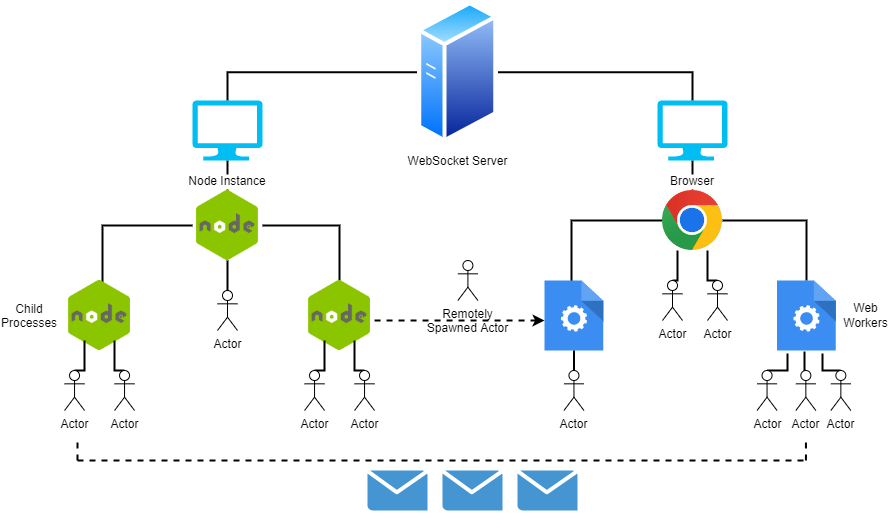
\includegraphics[width=390px]{resources/network.png}
        \caption{A Network of Devices with Multiple Processes Hosting Actors}
    \end{centering}\label{fig:network}
\end{figure}
\section{Actors on a Single Node.js or Browser Instance}
The first objective states that communicating actors can be spawned on either a Node.js or browser instance by developers. To support both environments, a framework is implemented for each, while providing a fully interoperable API. This enables code utilising the actor framework on one environment to work just as well on the other.
\subsection{Actor Design}
The design of the frameworks' actors is inspired by Gul Agha's paper~\cite{agha1985actors}. They are defined as computational agents which map communication to a behaviour, which may consist of spawning new actors, communicating with other actors, or defining a new behaviour for the next message. The behaviour of such actors is also said to be history sensitive, where previous behaviour executions may impact how the next communication is processed.

This definition prompts the API to allow for the creation of actors and the ability to send communications to the spawned actors. Communications sent to actors take the form of JavaScript objects due to their structural flexibility and conformity with Gul Agha's definition of a “tuple of values”~\cite{agha1985actors}. Actors are defined to have history sensitivity, which prompts each actor to hold a local isolated state, which also takes the form of a JavaScript object. The actor's behaviour takes the form of a conventional JavaScript callback function, which has the actor's state, message, and self address as function parameters. Since JavaScript provides first class functions, the behaviour definition is stored and called when required. This prompts for the following basic API using TypeScript's~\cite{typescript} syntax.
\begin{lstlisting}
interface ActorBehaviour {
    (state: object, message: object, self: ActorReference): void
}
spawn = (initialState: object, behaviour: ActorBehaviour): ActorReference
send = (actor: ActorReference, message: object): void    
\end{lstlisting}
The API returns an actor reference when one is spawned, which can then be fed into the send function as a parameter. The actor behaviour is invoked when processing each received message, and may manipulate the actor's state which is initially defined through a parameter passed into the spawn function. The actor behaviour may also use the API to spawn and communicate with other actors. The implementation of these two functions on the Node.js and browser environment fulfils the first defined objective in Section~\ref{section:objectives}. 
\begin{figure}[H]
    \begin{centering}
        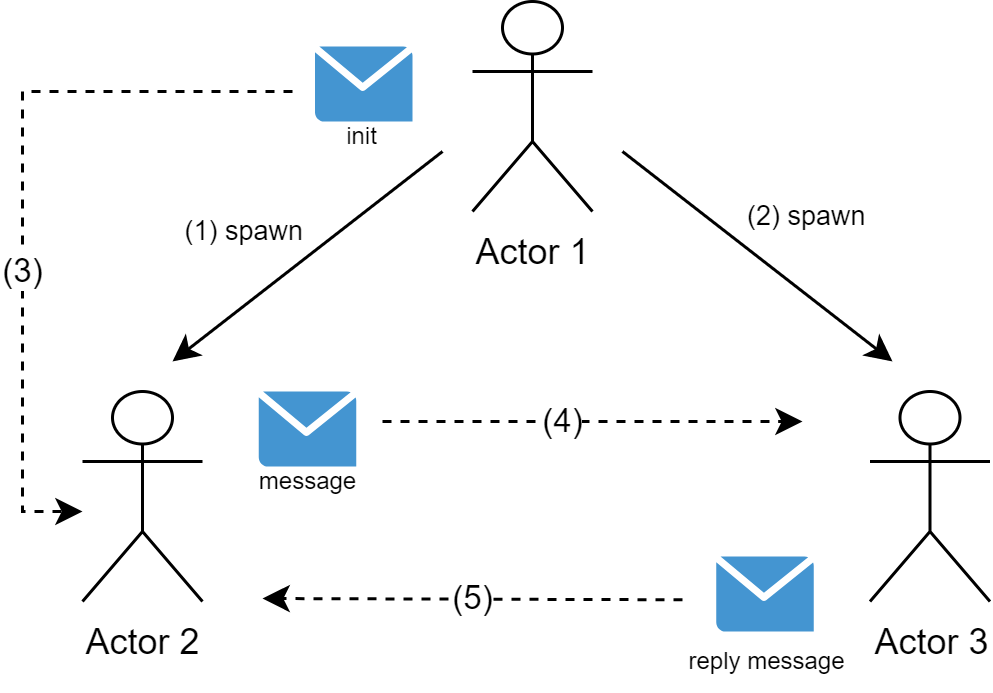
\includegraphics[width=270px]{resources/actors.png}
        \caption{Spawning Actors and Sending Messages}\label{fig:actors}
    \end{centering}
\end{figure}
Finally, a function to terminate an actor is provided, with the option for whether it should process its remaining messages. This function takes in an actor reference similar to the send function.
\begin{lstlisting}
terminate = (actor: ActorReference, force: boolean)
\end{lstlisting}

\subsection{Actor Anatomy}
The internal composition of an actor inside the framework is at the heart of the API's features. An actor takes the form of an object which contains its maintained state as well as its behaviour as an executable function. Each actor stores a name so that it can be uniquely identified in a local instance, and a `node' number which allows other clients to uniquely identify the actor's network location. Whether the actor processes incoming messages is also stored. The TypeScript interface below defines what an actor is composed of.
\begin{lstlisting}
//TypeScript object interface for an Actor
interface Actor {
    name: string,                       //generated using uuidv4
    node: number,                       //found in global variable
    state: { [key: string]: any },      //given by developer
    behaviour: ActorCallback,           //given by developer
    active: boolean                     //starts with true
}
\end{lstlisting}
When spawning an actor, the initial state and behaviour are defined by the developer. The name is automatically generated using a uuidv4 package~\cite{uuidv4}. All actors start off as active to indicate that they are processing messages. When returning the actor reference to the developer, an issue arises if the whole actor object is returned. Not only does it contain redundant information such as returning the state and behaviour that were just defined by the developer, it also undermines the concept of actor isolation. Since objects are passed by reference in JavaScript, the developer or other actors would be able to modify the actor's state and behaviour through its reference. To protect these attributes, only a subset of them are returned, defined by the following ActorReference TypeScript interface.
\begin{lstlisting}
interface ActorReference {
    name: string,   //identifies the actor on a local instance
    node: number    //identifies the client over the network
}
\end{lstlisting}

\subsection{Actor Runtime}
The JavaScript event loop~\cite{eventloopbrowser, eventloopnode} is responsible for executing the application code. The language's runtime has an event queue where each event is mapped to a function which processes that event. The event loop waits for the arrival of an event and processes the queue of events when there is a backlog in the event queue. Each event is processed to completion before other events are processed. The actor model also maps received messages onto functions, which act as message handlers. Therefore, the prototype's implementation takes advantage of the similar philosophies between the JavaScript runtime and the actor model.

The implementation acts as a wrapper of the JavaScript event loop. Once a message is received by an actor, it schedules the processing of the message on the JavaScript event loop. This is done by scheduling a microtask~\cite{microtasks}, which is an event queued to execute before the start of the next iteration of the event loop. The microtask is scheduled by creating a Promise which is immediately resolved. This behaviour is similar to using Node.js' \textbf{process.nextTick()}~\cite{nexttick}, which is more efficient than using the JavaScript's \textbf{setTimeout()} function, as it would otherwise schedule a macrotask which executes in the following iteration of the event loop.
\newpage
\begin{lstlisting}
//Code which schedules the processing of a received message
Promise.resolve().then(() => {
    if (message !== undefined && localActor.active)
        localActor.behaviour(localActor.state, message, { name: localActor.name, node: localActor.node });
})
\end{lstlisting}

JavaScript only has one microtask event queue, so the order in which messages are sent matches the order in which they are processed by the set of receiving actors. JavaScript also processes each microtask to completion before processing the next, thus ensuring that at most one actor is processing a message at any point in time on a single Node.js or browser instance.

\section{Actors on Multiple Node.js or Browser Instances}
\subsection{Actors on a Distributed Network}
So far, the actor framework implementation enables concurrent processing of messages on one browser or Node.js instance. It does not matter which actor processes their next message, or in which order the actor processes their messages, assuming that the actors are not overly dependent on their maintained isolated state. Concurrency~\cite{concurrencyjs, concurrency} implies that actors are potentially parallelisable, where multiple actors can process their next message in parallel and thus, have the potential to speed up the overall computation. The API must provide an intuitive way to establish a connection with other processes or devices to communicate with remote actors.

A peer-to-peer system is first considered to connect nodes which host actors. Each peer would have a list of nodes to establish connection with. While this would eliminate the additional network hop introduced by an intermediate server, the number of connections performed would be $n!$ if each node is listening for connections and connects to every other node. Furthermore, manually entering which peers each node needs to establish connection with is tedious. Instead, the prototype opts for a central WebSocket server for distributed networking, as each node can communicate with the rest of the network, using only $n$ connections.

\subsection{Implementing a WebSocket Server}
The WebSocket server expects a fixed number of $n$ connected clients before it starts accepting communication to be forwarded between nodes. The server logic was developed separate from the actor framework, and assumes that connections are not terminated in the duration of its runtime. The WebSocket server assigns a unique identifier to each connected client which is broadcasted when the server establishes the expected number of connections. This allows developers to uniquely identify clients on the WebSocket network.

\begin{figure}[H]
    \begin{centering}
        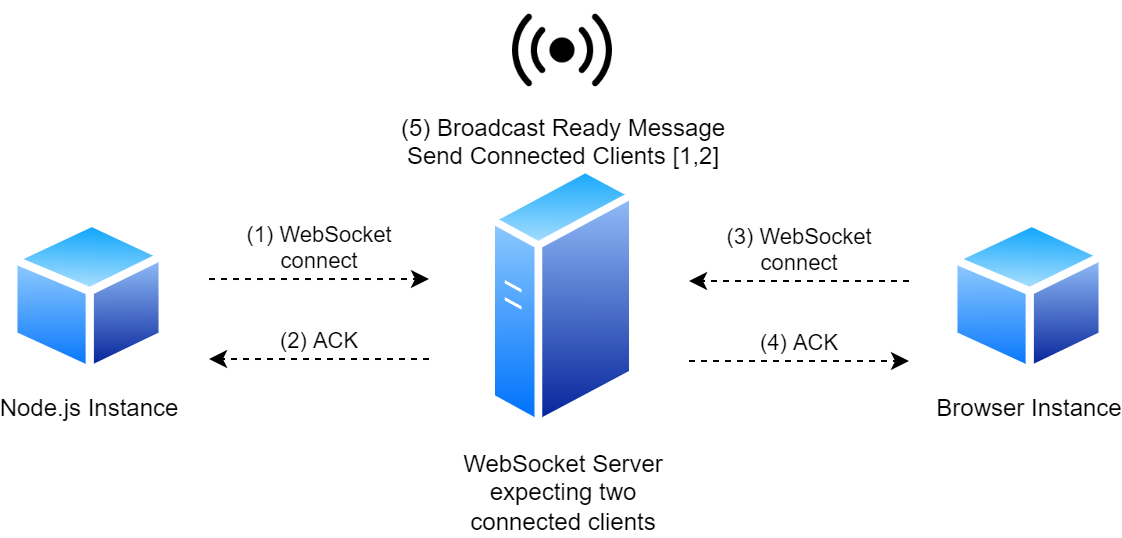
\includegraphics[width=\textwidth]{resources/websocketconnection.png}
        \caption{WebSocket Server Connecting Node.js Instance to a Browser}\label{fig:websocketconnection}
    \end{centering}
\end{figure}
 
This mode of establishing communication between nodes has several advantages and disadvantages. The centralised WebSocket server effectively creates a barrier, which lifts when the expected number of clients are connected and can communicate with each other. Once the number of expected clients connect, each client is granted communication with the entire network at the cost of the network hop over the WebSocket server. The centralised server also simplifies the logic of uniquely identifying each connected client, which is a simple iterative naming scheme in the order in which clients connect. Connecting to the server should take the form of an API function call which returns a Promise. This Promise resolves when the server broadcasts to the client that it is ready to forward information to the other connected clients.
\begin{lstlisting}
init = (url: string, timeout:number): Promise<object>
\end{lstlisting}

\subsection{Remote Spawning Mechanism}
The developer must be able to refer to actors which exist in remote nodes. API functionality to remotely spawn actors on other nodes would address this requirement as it would allow for one instance to get references to actors it remotely spawned. Security is potentially an issue since actors could be spawned remotely on machines by malicious peers. However, it allows for expressive programs which can centrally load balance work on a distributed network by sending messages to the remote actors using the obtained references through remote spawning.
\begin{lstlisting}
spawnRemote = (node: number, state: object, behaviour: ActorBehaviour, timeout: number): Promise<ActorReference>
\end{lstlisting}

The \textbf{spawnRemote} function sends a request to spawn an actor to the remote node. The request has embedded within it the string representation of the actor behaviour, which is reconstructed as a function on the recipient end. On the recipient's side, the client spawns an actor with the sent behaviour and initial state. It locally generates the spawned actor's name and embeds it in an acknowledgement sent to the remote spawner. Once this acknowledgement is received by the spawner, it constructs the actor reference using the received actor name, and resolves the Promise.

\subsection{Local Parallelism on Multicores}
The WebSocket server provides distribution for any Node.js or browser client wishing to communicate with actors hosted on other connected clients. However, a developer might want to host multiple instances on a local multicore device to make up for JavaScript's single-threaded runtime when distributing actors. The WebSocket server requires an intermediary network hop as well as the network layer, both of which can be avoided by using Node.js Cluster~\cite{nodejs, cluster} and browser Web Workers~\cite{webworkers}. These methods rely on inter-process communication (IPC), which allows direct communication between the spawner and the workers over shared memory. Each of the spawned workers can also be treated as separate instances when connected to the WebSocket server for communication with remote devices.

\begin{figure}[H]
    \begin{centering}
        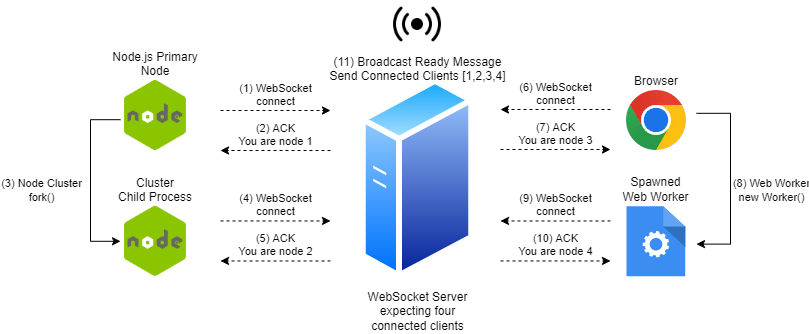
\includegraphics[width=\textwidth]{resources/websocketconnectioncomplex.png}
        \caption{WebSocket Server Connecting Different Types of Processes}\label{fig:websocketconnectioncomplex}
    \end{centering}
\end{figure}

This would require changing the API's \textbf{init} function to allow the developer to specify the number of additional workers to spawn and connect to the WebSocket server, resulting in the function definition below. The default number of workers is set to 0, where the instance would not spawn any workers.
\begin{lstlisting}
init = (url: string, timeout: number, numWorkers: number = 0): Promise<object>
\end{lstlisting}

When the developer spawns child processes or Web Workers, each of the spawned workers send the network number assigned to them by the WebSocket network to the spawner (primary node). The primary node then sends each of the spawned workers of their neighbouring spawned processes' network numbers. This happens so that spawned workers can identify their neighbours and communicate with them by sending messages to the primary node instead of the WebSocket server. The primary node forwards the message to the destination worker using the Node.js Cluster or Web Worker API instead of the WebSocket network to avoid the network stack. If the actor resides on a separate device or group of spawned processes, it resorts to using the WebSocket network.
\section{Location Transparency}
Now that Node.js Cluster child processes and browser Web Workers have been introduced and incorporated into the API's design, the send function would benefit from location transparency. This would mean that the developer does not need to specify whether the actor resides in a spawned Web Worker or Node.js child process, as well as whether it is a local or remote actor. This is done by embedding the assigned network number as well as the actor's unique name inside the actor reference returned by the API's spawning functions. The actor name is generated using UUIDv4~\cite{uuidv4}, which generates universally unique IDs with a high probability.
\begin{lstlisting}
interface ActorReference {
    name: string,
    node: number
}
\end{lstlisting}
Using the returned ActorReference object from the \textbf{spawn} or \textbf{spawnRemote} function, an actor can be uniquely identified across the network. The developer can pass the actor reference as a parameter to the \textbf{send} function to send that actor a message. Internally, the framework looks at the actor reference's network number and chooses the fastest available link. 

If the actor's network number matches the sending client's network number, then it queues the local actor's behaviour on the runtime's event queue. If the actor resides in a remote node, it creates a payload to send over the network. Since the IPC connections are faster than using a WebSocket connection with an intermediary hop, the client first checks if the remote actor resides in a neighbouring process which can be communicated with using IPC. If the sending client is the primary node, it can directly send the message to the spawned worker. Spawned workers can communicate with each other by sending messages to the primary node, which forwards them to the recipient worker. If the actor resides in a remote node that is not a neighbouring process, it sends the message to the WebSocket server for routing.
\begin{figure}[H]
    \begin{centering}
        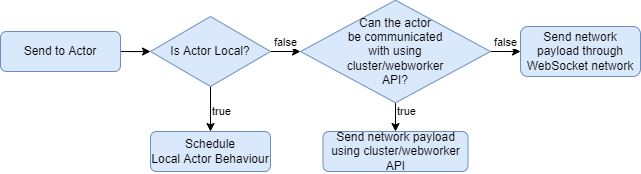
\includegraphics[width=\textwidth]{resources/communication.png}
        \caption{Flowchart for Choosing which Link Based on Actor Location}\label{fig:communication}
    \end{centering}
\end{figure}

When remotely spawning actors using the \textbf{spawnRemote} function, the developer provides the network number which was assigned to a specific client by the WebSocket server. The client which possesses this network number receives a request to spawn the actor. The framework internally resolves whether this client is a neighbouring instance which can be communicated with through IPC, or a remote instance which requires the WebSocket server's involvement. The developer need not be concerned with whether the client which spawns the actor is local or remote, or where the client resides in on the distributed network.

The convenience of location transparency is provided through the WebSocket server, which provides unique names to each of the connected clients. Actors on different clients in the network communicate with each other through the WebSocket server, which routes each of the messages accordingly. This comes at the cost of having each of the distributed nodes relying on a potentially failing central point.
\chapter{Evaluation}\label{chap:evaluation}
This chapter evaluates the developed prototype's performance when executing computationally intensive tasks. Savina~\cite{savina} is a benchmark suite defined for actor-based systems which is implemented using this disseration's framework. Section~\ref{section:microbenchmark} explores each of Savina's micro-benchmarks, which measure overheads introduced when using the framework's basic functionality. Section~\ref{section:parallel} explores parallel benchmarks which expect a linear increase in performance with each added working actor. Benchmark configurations as well as raw data can be found in Appendix~\ref{appendix:results}. 

Measures were taken to address various threats to validity of the obtained results, mainly centered around ensuring that a stable computing environment was provided. Benchmarks were mainly run on a fresh Ubuntu install to minimise the number of running background processes. Hyper-threading was disabled to ensure that each single-threaded JavaScript instance makes use of exactly one core. Each benchmark is run multiple times to observe the variance and standard error when extracting the average result.

Unless otherwise stated, the following hardware and software was used to run the benchmarks.
\begin{itemize}
    \item OS --- Ubuntu 20.04 focal (64 bit)
    \item CPU --- Intel Core i7--1065G7. 4 cores at 3.9GHz with hyper-threading disabled
    \item RAM --- LPDDR4 16GB (2$\times$8GB) at 4267MHz
    \item Node.js --- v16.14.0
    \item Google Chrome --- v100.0.4896.88 (Official Build)
\end{itemize}
\newpage
\section{Micro-Benchmark Performance}\label{section:microbenchmark}
\subsection{Comparing Local Node.js to Browser Performance}
The Savina benchmark suite defines micro-benchmarks which test specific actor runtime features. Figure~\ref{fig:micro} compares the execution times between the browser and Node.js implementations of Savina's micro-benchmarks. The diagram is followed by an explanation and analysis of each of the executed benchmarks from left to right.
\begin{figure}[H]
    \begin{centering}
        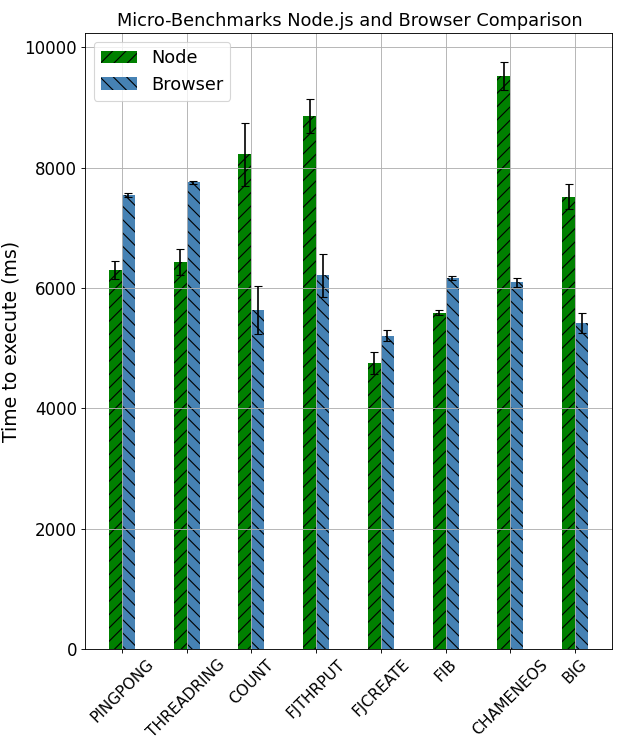
\includegraphics[width=270px]{resources/micro.png}
        \caption{Node.js and Browser Comparison for Micro-Benchmarks}\label{fig:micro}
    \end{centering}
\end{figure}

\begin{itemize}
\item Ping-Pong – Two actors are spawned, which send messages to each other. Every time one actor receives the message, it decrements the integer value it receives and sends it back to the sender. This mainly tests the send functionality on a local instance, with Node.js being slightly faster at sending the same load of messages.
\item Thread-Ring – Similar to Ping-Pong, the token containing the decrementing integer is now forwarded across $N$ actors. Instead of the message being sent back and forth, it is now forwarded to the next actor on the ring. The performance is nearly identical to that of Ping-Pong, as the framework does not perform context switching between actors. The JavaScript event loop merely executes the queued functions which process the actors' messages. The initial decrementing integer value (which determines the load) was set to the same as the Ping-Pong benchmark.
\item Count – This benchmark sends $N$ messages to a single actor and waits for the actor to process all of the received messages. It tests the time taken for $N$ messages to be sent and then processed by an actor. Since the framework relies on the event loop, each and every sent message gets queued in the event queue. Node.js is considerably slower than the browser implementation with a high standard deviation on both environments. This may be due to the operating system having to allocate a considerable amount of memory in a short amount of time when queuing a large number of messages.
\item Fork-Join-Throughput – This benchmark starts by sending $N$ messages to $K$ actors in a round robin fashion instead of one counter actor. Similar performance is achieved to that of the Count benchmark when sending the same number of messages.
\item Fork-Join-Create – This benchmark creates $N$ actors and sends each spawned actor a single message. It tests the spawning, sending, and terminate functionality of the framework by spawning actors and sending one message to each, which causes the actors' termination. The performance is similar between the two environments, with the browser being slightly slower.
\item Fibonacci – This benchmark creates new actors to recursively compute the n'th iteration of the Fibonacci sequence. It differs from Fork-Join-Create as the actors spawned to execute larger iterations of the Fibonacci sequence live longer than those executing smaller iterations. Similar relative performance is achieved between Node.js and browser.
\item Chameneos – This benchmark spawns a single mall actor and $N$ Chameneos actors. Chameneos actors send to the mall actor numerous requests to be matched with other Chameneos actors. The benchmark tests contention on the mall actor, as it needs to match pairs of Chameneos while they create a considerable amount of noise in the event queue. When the mall matches two Chameneos which sent a request, they will exchange a state between each other. A large number of messages are queued, making this benchmark memory intensive, which may be the reason Node.js is significantly slower than the browser, similar to the Count and Fork-Join-Throughput benchmarks.
\item Big – This benchmark involves $N$ actors picking random actors to send messages to. The recipient of the actor will then reply to the sender with a reply message. This tests many-to-many actors passing messages to each other, with node achieving slower performance than browser.
\end{itemize}
The Chameneos benchmark tests many actors sending messages to one actor, while Big has many actors sending messages to random actors. This does not make a difference to the actor framework model as the concept of an actor is merely an abstraction. The framework acts as a wrapper around the runtime's single-threaded event loop and queue. Rather than all actors having their own mailbox and thread of control, a single JavaScript event loop executes functions stored on a single event queue with the actor's state and received message as the context of its behaviour. Consequentially, similar performance is achieved for both benchmarks when comparing between the browser and Node.js environments.

Ping-Pong and Thread-Ring are another pair of benchmarks which execute the same effective load using this dissertation's framework. The Thread-Ring benchmark tests for any overhead introduced by having more actors forwarding the message. However, each actor is merely a saved object in the framework which stores the actor's state and behaviour and does not have any bearing on its runtime performance when sending and processing messages.

Count, Fork-Join-Throughput, Chameneos and Big each queue a large number of messages on the JavaScript event queue. Node.js consistently performs slower than the browser when holding a large number of actor messages on its event queue. The browser may be more efficient at storing a large number of events on its event queue than Node.js.
\subsection{Node.js and Browser Micro-Benchmark Load Scaling}
\begin{figure}[H]
    \begin{centering}
        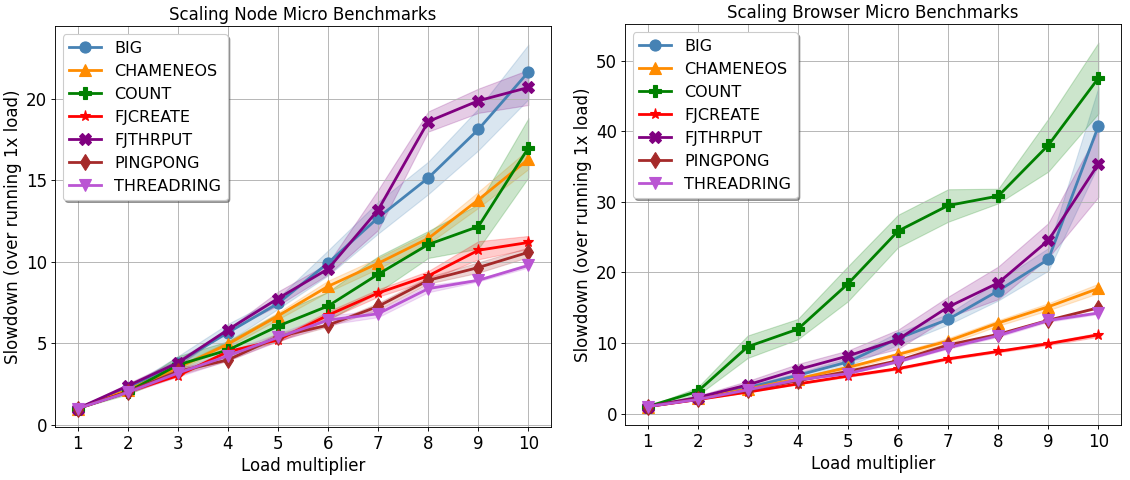
\includegraphics[width=\textwidth]{resources/load_scaling.png}
        \caption{Node.js and Browser Micro-Benchmark Load Scaling}\label{fig:load_scaling}
    \end{centering}
\end{figure}
One can observe that Big, Chameneos, Count and Fork-Join-Throughput have the worst scaling when increasing load over both environments. All four of these benchmarks involve large message queues, suggesting that JavaScript performs slower when more messages are in the event queue. The browser demonstrated approximately twice the slowdown for some of the benchmarks, which may be the result of less RAM being available on a browser instance than that of Node when queuing a large number of messages.
\subsection{Comparing Communication Links}
The Ping-Pong and Fork-Join-Create benchmarks were tested on a network using different links. In this comparison, the Fork-Join-Create benchmark only involves the remote spawning of actors without them executing any behaviour, such as terminating. This way, the comparison narrows down the performance to sending messages through the Ping-Pong benchmark and remote spawning through Fork-Join-Create.
\begin{figure}[H]
    \begin{centering}
        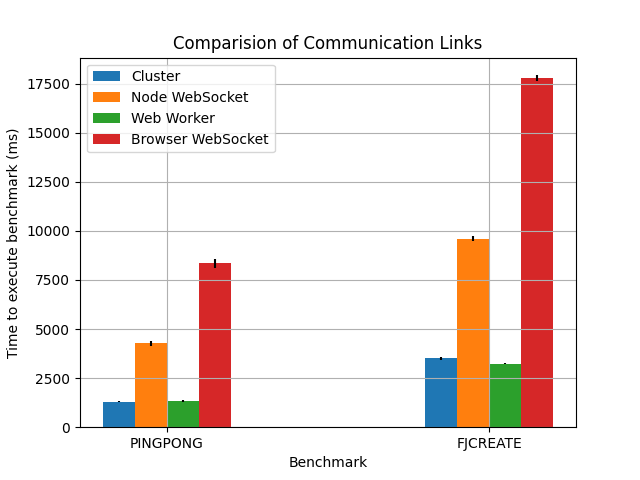
\includegraphics[width=300px]{resources/link.png}
        \caption{Comparison of Communication Links}\label{fig:link}
    \end{centering}
\end{figure}
Across both benchmarks, Cluster and Web Workers are nearly identical in performance. Node.js uses an npm package to interface with the WebSocket server while the browser uses the available WebSocket functionality on JavaScript. The browser is slower when communicating through the WebSocket link in both cases. 

The WebSocket links are slower than the IPC alternative (Cluster and Web Workers) since they involve the network stack and introduce an additional network hop over the WebSocket server. Cluster and Web Workers use a direct link which is made between the spawner and the spawned worker; hence the message is not forwarded by an intermediary node. WebSocket performance would be improved if peer-to-peer connections between distributed instances were established.

Furthermore, the number of actors which are remotely spawned in Fork-Join-Create is equal to the number of messages sent in the Ping-Pong benchmark. The Fork-Join-Create benchmark is about twice as slow since it involves sending twice the number of messages over the network. The first message is a request sent to the remote instance to remotely spawn an actor. When the remote instance spawns the actor, it sends an acknowledgement message with the actor's address embedded within.
\subsection{Comparing with Existing Implementations}
\begin{figure}[H]
    \begin{centering}
        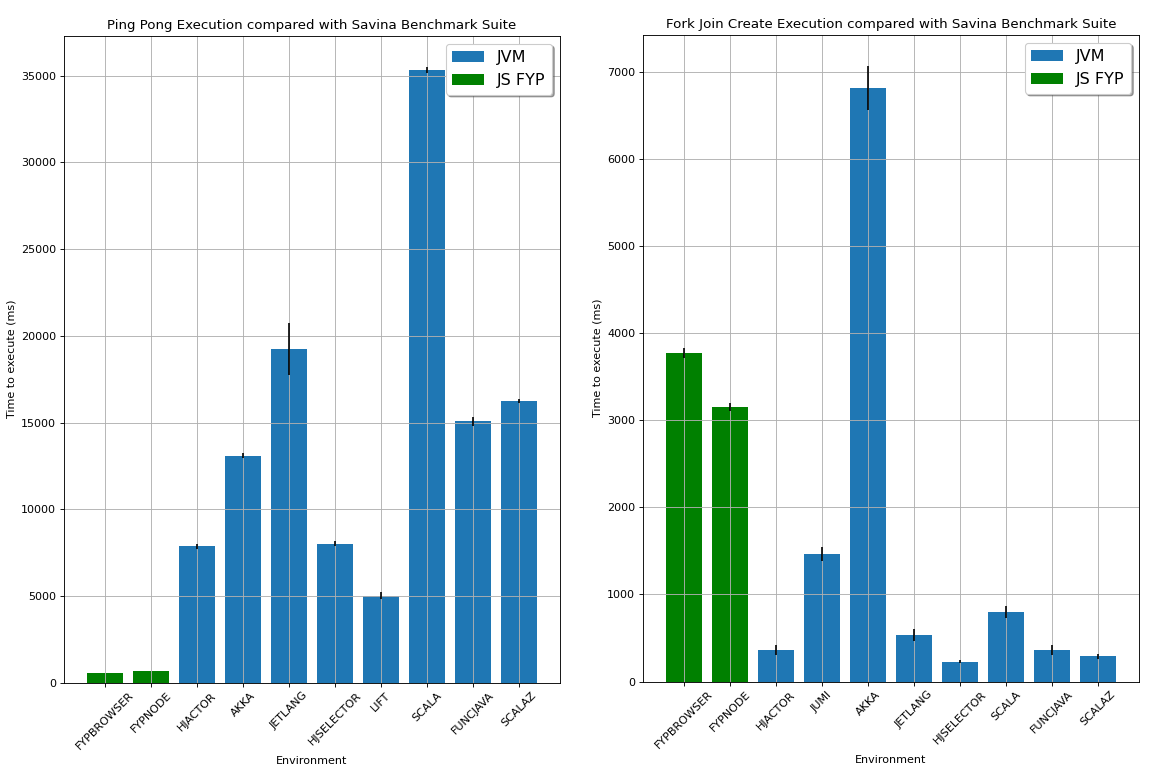
\includegraphics[width=\textwidth]{resources/savina.png}
        \caption{Savina Benchmark Comparison with other Implementations}\label{fig:savina}
    \end{centering}
\end{figure}
This dissertation's framework performs the fastest when messages are sent between actors. This is effectively the speed at which JavaScript can create and immediately resolve Promises followed by a minimal amount of work to create the next Promise. Nact is much slower as it maintains a mailbox of messages using a queue, and includes logic, which checks if an actor is busy processing a message or not. This may be due to its features to persist actors and events on a database, which requires the framework to keep track of the current actor queues. This dissertation's framework benefits from acting as a wrapper around the event loop, as it directly makes use of the event queue to schedule tasks rather than performing the additional task of manipulating objects in memory. The JVM implementations prove to be more costly in general, where Scala required the throwing of exceptions~\cite{savina} to maintain the benchmark's control flow.

The framework does not perform as well when spawning actors, ranking in the fourth worst execution times when compared with the JVM implementations and Nact.  Spawning actors in Nact ran much slower than this dissertation's framework due to Nact's more complex logic involved when creating an actor, which may be attributed to Nact's support for hierarchies of actors. Meanwhile, this dissertation's framework simply keeps record of the actor in a global object and returns the reference to that actor. Akka performed the slowest in the JVM category, which is in line with the benchmarks executed in Savina's paper.  However, no reasons have been given for Akka's slow actor creation.

These benchmarks were also implemented for Spiders.js. This framework failed to create the number of actors spawned when benchmarking Fork-Join-Create (one million actors). This is due to the framework creating a new child process for each spawned actor to grant them their own thread of control, causing each actor to be memory intensive. Spiders.js was also dramatically slower when running the Ping-Pong benchmark compared to its JavaScript and JVM counterparts. A modified version of the provided Ping-Pong example was used to implement this benchmark, and poor processor utilisation was observed when sending messages between the actors involved. Running the benchmark also slowly and continuously allocated a considerable amount of RAM, which should not be the case when the number of actors is constant, and not more than one message is queued at a time.
\section{Parallel Performance}\label{section:parallel}
\subsection{Shared Memory Parallelism}
This subsection first demonstrates the parallel nature of the benchmarks and its results, followed by a mathematical explanation for each of the benchmarks.
\subsubsection{Performance Results}
The Savina benchmark suite includes parallel benchmarks where multiple actors perform computation in parallel to complete a task. Each of the explored parallel benchmarks in this dissertation benefit from master-worker parallelism, where a master actor farms tasks to worker actors, which will start execution in parallel. Then, the workers report their results to the master, which aggregates the collected data, producing the final result. The framework is tested by first executing the benchmark using only one master and one worker in separate runtimes, where the worker is limited by JavaScript's single-threaded nature.  Next, two workers are spawned on separate runtimes, each of which is ideally assigned half of the computational load by the master. Since the framework is tested on a system which houses four cores, the benchmarks are scaled up to four worker runtimes running in parallel. The speedup introduced over running on one worker is tested and plotted in Figure~\ref{fig:shared_memory_speedup}, where near linear results can be observed.
\begin{figure}[H]
    \begin{centering}
        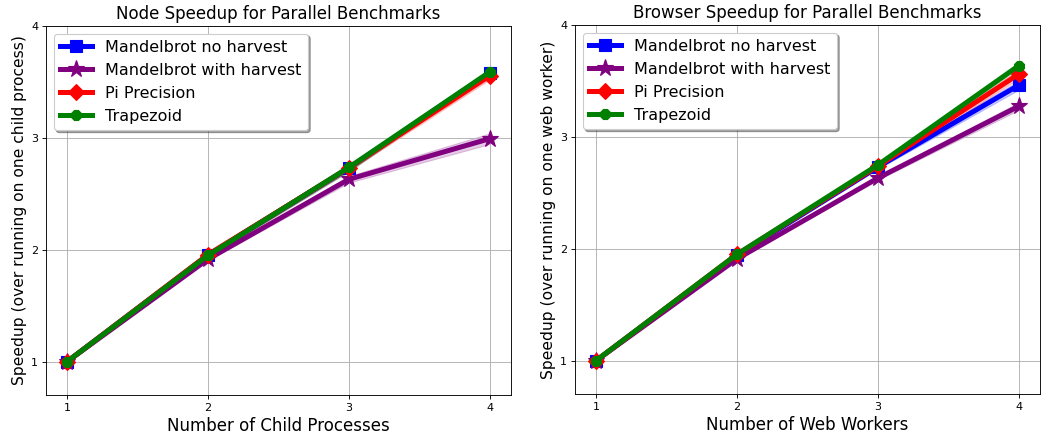
\includegraphics[width=\textwidth]{resources/shared_memory_speedup.png}
        \caption{Node.js and Browser Comparison for Shared Memory Speedup}\label{fig:shared_memory_speedup}
    \end{centering}
\end{figure}
\subsubsection{Mandelbrot}
The Mandelbrot benchmark is not part of the Savina benchmark suite. Generating the Mandelbrot set~\cite{mandelbrot} is highly parallelisable as each pixel can be independently computed using a set of provided constants. 
\begin{itemize}
    \item The worker actors execute iterations of $z_{n+1}$ = $z_{n}^{2}+c$ where $z_0 = 0 + 0i$
    \item $c, z \in \mathbb{C}$. $n \in \mathbb{Z},$ $n \ge 0$
    \item $c$ is determined by the position of the pixel
    \item If $|z_n|> 2$ it is said to be unbounded and will generate a lighter pixel colour if $n$ is small. If it performs a set number of iterations and it is still bounded $(|z_n| \le 2)$, it yields a darker colour.
\end{itemize}

\begin{figure}[H]
    \begin{centering}
        
\includegraphics[width=215px]{resources/mandelbrot.png}
        \caption{Mandelbrot Set Image Generated using Distributed Actors}
    \end{centering}
\end{figure}
Black pixels take longer to compute than white pixels, as the maximum number of iterations need to be performed to verify that the point in the Mandelbrot set remains bounded. For this reason, Mandelbrot could not be split into even pixel chunks amongst workers as chunks which have more black pixels would take considerably longer to execute, resulting in some workers finishing faster than others, thus reducing efficiency. The master could compose each task to be a single row where once a worker is finished with a row, it is assigned the next required row. However, this would result in considerable message overhead as the number of messages exchanged between the master and its workers would be twice the image's height. A balance is struck between minimising message overhead and distributing even chunks by assigning smaller chunks to each worker. When the worker reports the results back, it is assigned the next required chunk.

When workers do not report back the generated pixels to the master, the speedup goes up to 3.5 with four running workers. The slowdown may be attributed to the fact that the master is running on its own process (thus using five processes on four cores), as well as any other processes and daemons running on the operating system, which may have prevented the benchmark from fully utilising the CPU. The distributed chunk sizes may not have been optimal resulting in some workers finishing earlier than others. There were also instances where workers were idle while waiting for the next task to be assigned by the master. When harvesting the chunk's pixel data from the workers, one can note that Node.js had more significant slowdown than the browser on four worker processes.
\subsubsection{Pi Precision and Trapezoidal Approximation}
The value of pi computation as well as the trapezoidal approximation benchmarks involve a master actor distributing iterations of mathematical computation to worker actors.

The value of pi is approximated using Equation~\ref{eq:pi}, which is defined by the Savina benchmark suite. The iterations of the summation can be distributed and parallelised amongst multiple worker actors.
\begin{equation} \label{eq:pi}
\pi=\sum_{n=0}^{\infty}\left(\frac{4}{8n+1}-\frac{2}{8n+4}-\frac{1}{8n+5}-\frac{1}{8n+6}\right) \left(\frac{1}{16} \right)^n
\end{equation}
Trapezoidal approximation can also be distributed to perform the approximate integral of Function~\ref{eq:trapfunc} specified by the Savina benchmark.
\begin{equation} \label{eq:trapfunc}
f(x)=\frac{1}{x+1}\cdot\sqrt{1+e^{\sqrt{2x}}}\cdot \sin\left(x^3-1\right)
\end{equation}
This is done by executing Equation~\ref{eq:trapapprox} with respect to $f(x)$ using $N$ intervals. Each worker executes smaller bounds of the integral of $f(x)$ which are add up by the master to compute the full integral.
\begin{equation} \label{eq:trapapprox}
\int_{a}^{b}f(x)dx\approx\frac{b-a}{N}\left[ \frac{f(a)+f(b)}{2}+\sum_{k=1}^{N-1}f\left( a+k\cdot\frac{b-a}{N} \right) \right]
\end{equation}
\subsection{Distributed Memory Parallelism}
The following benchmark experiments with having actors hosted across distributed memories. A Raspberry Pi 4 is used to host a WebSocket server, which handles the forwarding of messages between the connected devices. The scaling of the Mandelbrot benchmark without harvesting pixel data over Node.js and browsers has already been explored up to four worker instances over shared memory. Figure~\ref{fig:distributed_memory_speedup} shows the speedup introduced when connecting two devices to the Raspberry Pi WebSocket server. The connections are made locally using a 5GHz WiFi connection, with an observed speed of 50Mbps when transferring data to and from the server. The device that was used to execute the previous benchmarks is the first device which is connected to the device, while the second device is described as follows: 
\begin{itemize}
    \item OS --- Windows 10 Home (64 bit)
    \item CPU --- Intel Core i5--10500 6 cores up to 3.10GHz with hyper-threading enabled
    \item RAM --- DDR4 32GB (4$\times$8GB) at 2666MHz
    \item Node.js --- v16.14.0
    \item Google Chrome --- v101.0.4951.67 (Official Build) (64-bit)
\end{itemize}
In addition to the four workers and master hosted on the four-core device, new workers are incrementally added and connected to the WebSocket server on the new device. While avoiding data harvesting to minimise the network dependency, one can observe a consistent speedup when adding more workers on the second device, with Node.js achieving slightly better speedup with a larger number of workers. Despite network overhead being introduced when distributing actors over the network, the second device makes up for this with its faster processing time.
\begin{figure}[H]
    \begin{centering}
        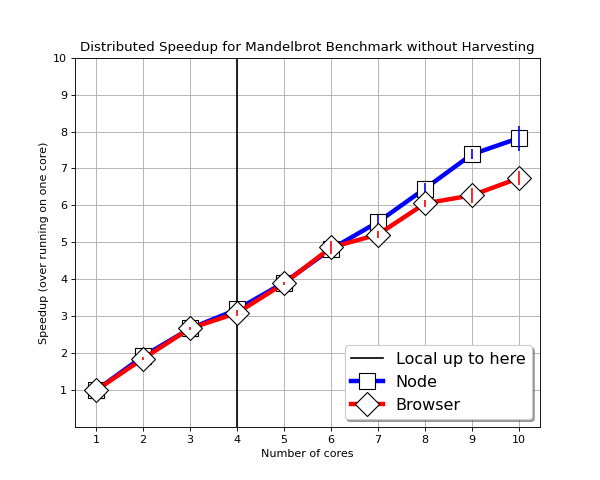
\includegraphics[width=280px]{resources/distributed_memory_speedup.png}
        \caption{Node.js and Browser Comparison for Distributed Memory Speedup}\label{fig:distributed_memory_speedup}
    \end{centering}
\end{figure}
\section{Case Study}
While the quantitative analysis of the framework yielded sane results, the framework's ease of use is important for the developers making use of the API when engineering actor-based systems. This section focuses on two case studies which make use of the framework to create two communicating actors on a single instance as well as over a distributed network. The examples presented below work for both the Node.js and browser environments due to the framework implementations being fully interoperable. A manual for the frameworks' API can be found in Appendix~\ref{appendix:manual}.
\begin{lstlisting}    
import actors from 'actors.js';
const { init, spawn, spawnRemote, terminate, send} = actors

const pingPongBehaviour = (state, message, self) => {
    send(message.replyTo, {val: message.val-1, replyTo: self});
    if(message.val-1 < 0)
        terminate(self)
    else    
        console.log(message.val);
};
\end{lstlisting}
The code snippet above first imports the framework by using JavaScript ES6 imports. Lines 4--9 define an actor behaviour, which immediately sends a message to the sender, including a reference to itself as well as the value it received subtracted by 1. It then checks if the value it received is less than 0, and if so, the actor terminates itself. Otherwise, it outputs the received value. Each of the examples presented in this case study assume that the framework is imported and that the actor behaviour is predefined. 
\subsection{Single Instance Actor Based System}
When making use of actors in a single instance, the developer is required to make use of three API functions taking in two parameters each. These functions allow the developer to \textbf{spawn} actors, \textbf{send} messages to them, and \textbf{terminate} them to free up memory. The example below makes use of these three API functions to build two communicating actors for a specified load.
\begin{lstlisting}    
const pingActorRef = spawn({}, pingPongBehaviour);
const pongActorRef = spawn({}, pingPongBehaviour);
send(pingActorRef, {replyTo: pongActorRef, val: 5});
\end{lstlisting}
Two actors are spawned with this behaviour, and the system is initialised by sending one of the actors the reference of the other actor, as well as a value of 5. The first actor outputs the values 5, 3 and 1, while the second actor will output the values 4 and 2, as they send each other decrementing values until both terminate when receiving a value of 0 or less.
\subsection{Distributing Parallel Actors over a Network}
The functionality demonstrated above can be easily replicated without the framework by using function calls and JavaScript Promises. However, by using the actor framework API, one can distribute the ping and pong actors across separate machines with minimal change in the code's logic. The provided WebSocket server needs to be started and set to expect three connected clients. 

One machine connects to the WebSocket server and uses the \textbf{spawnRemote} function instead of \textbf{spawn}, which requires an additional parameter to specify which remote machine spawns the actor.
\newpage
\begin{lstlisting}
init('ws://localhost:8080').then(async ready => {
    const pingActorRef = await spawnRemote(2, {}, pingPongBehaviour);
    const pongActorRef = await spawnRemote(3, {}, pingPongBehaviour);
    send(pingActorRef, {replyTo: pongActorRef, val: 5});
});
\end{lstlisting}

The two machines which are remotely instructed to host the ping and pong actors respectively simply connect to the server.
\begin{lstlisting}
init('ws://localhost:8080')
\end{lstlisting}

Once all clients connect to the server, the server lifts the barrier and thus resolves the Promise on the first machine. The first machine then sends requests to spawn actors on the remote machines, which only need to connect to the server. Due to location transparency, the \textbf{pingPongBehaviour} function remains unchanged, as the framework internally resolves which communication link needs to be used when replying to the actor. In this case, the actors communicate with each other over the WebSocket link.

The developer can pass in additional parameters to specify the timeout to wait for the server to lift the barrier, as well as how many additional Web Workers or Node.js child processes the instance should spawn and connect to the WebSocket network. The code snippet below spawns the ping actor on one spawned worker and the pong actor on another. This is done by passing additional parameters to the \textbf{init} function. The spawned workers take the form of Web Workers or child processes, depending on the environment it is run on.
\begin{lstlisting}
init('ws://localhost:8080', 10000, 2).then(async ready => {
    if(ready.yourNetworkNumber === 1){
        const pingActorRef = await spawnRemote(2, {}, pingPongBehaviour);
        const pongActorRef = await spawnRemote(3, {}, pingPongBehaviour);
        send(pingActorRef, {replyTo: pongActorRef, val: 5});
    }
});
\end{lstlisting}
With this simple change, the actors now communicate through each other using IPC through the primary node to avoid the WebSocket server additional hop and network stack. An if statement is placed as each spawned worker will run the same code, and only one node should be remote spawning to other nodes.

This section illustrated the minimal code changes required to scale an application from a single instance to using a distributed network or a multicore system through the use of only five API functions.
\chapter{Conclusions and Future Work}\label{chap:conclusions}
The prototype successfully provides an intuitive, scalable, and fairly performant JavaScript implementation of the actor model for both the Node.js and browser environments. The functionality is exposed through an API as a collection of functions which abstract the concept of actors as well as the use of numerous communication links for distributed and parallel programming. The developed framework exploits the similarities between Gul Agha's~\cite{agha1985actors} definition of the actor model and JavaScript's event loop~\cite{eventloopbrowser, eventloopnode} to minimise the slowdown introduced when utilising the framework. 

Each of the dissertation's four objectives were fully achieved. The two frameworks allow developers to spawn and send messages to actors on local Node.js and browser instances respectively. Messages are processed through the execution of the predefined behaviour of actors (Objective 1). Using several web technologies, developers are not limited to a single instance when spawning actors, as they can spawn actors on remote browsers and Node.js instances (Objective 2). Once actors are spawned either locally or remotely, the framework internally handles local and remote communication without additional input required by the user (Objective 3, location transparency).

The framework was evaluated using both qualitative and quantitative analysis (Objective 4). Quantitative benchmarks yielded sane results when using the Savina actor benchmark suite~\cite{savina}. The separate Node.js and browser frameworks demonstrated similar performance in most cases, with reasonable standard error. Furthermore, the provided communication links performed consistently across the different benchmarks. The performance of the prototype was compared with existing JavaScript and JVM implementations, achieving the fastest times for sending messages between actors and having them subsequently processed. The speedup of parallel actors was observed to be close to the ideal linear speedup when utilising up to four cores, and achieved a reasonable speedup when distributed actors were introduced. 

The developed actor framework is not without its limitations. Distributed clients must connect to a provided WebSocket server to communicate with their peers. Each client must wait for the expected number of clients to connect before being allowed to communicate with each other, and communication over the server introduces an intermediary network hop. The distribution of actors could be done using peer-to-peer WebSocket connections at the cost of more complex synchronisation and requiring each client to listen for connections.

The framework also lacks quality of life features such as the ability to freeze actors and persist them to a file. Persisted actors could then be spun up in different environments or runtimes, or serve as backup for when an actor reaches an undefined state. The framework could also provide the means to implement a hierarchy of actors, where the termination of an actor would automatically terminate its children, or have actors supervise other actors to provide fault tolerance~\cite{faulttolerance, lebrun}.

Grounded in the actor model's theory, the prototype complements the internet's distributed environment made up of machines hosting multicore processors, while taking advantage of JavaScript's far-reaching availability through the use of server-side applications and browsers. It provides a solution for developers to fully utilise the hardware present in multiple devices running vastly different operating systems with varying restrictions, given that a JavaScript runtime is present.

%%\pagestyle{umpageback}
{%backmatter % comment this out otherwise are not numbered
    % Bibliography
    \if@openright\cleardoublepage\else\clearpage\fi
	%% For references use IEEE style [5] or Harvard style [6]
    \bibliographystyle{IEEEtran} %% specific plainnat does not show url for articles
    % Use something like https://flamingtempura.github.io/bibtex-tidy/ to clean all your bibtex entries
    {\scriptsize\bibliography{references}}
	\printindex
}

\appendix
\chapter{Media}\label{appendix:media}
This dissertation's artefact can be accessed through the following means:
\begin{itemize}
\item GitHub Repository --- \url{https://github.com/Android2771/actors-fyp}. One may request access to the private repository by getting in contact with the author.
\item Google Drive Link --- \url{https://drive.google.com/drive/folders/17SXGm4jH9wzs7wU5a3R5CNEewjWGqoVh?usp=sharing}
\item Any provided physical media with the dissertation such as a CD
\end{itemize}

The artefact was also sent to the ICT Administrator. The artefact contains the following contents:
\begin{itemize}
\item A soft-copy of this report
\item README containing instructions to make use of the project
\item Actor framework source code for the Node.js and Browser environments
\item WebSocket server implementation
\item Benchmarks implemented using the developed frameworks
\item Python scripts to visualise data retrieved from running benchmarks
\end{itemize}

The Google Drive link also contains a demo in video format which runs a number of the provided benchmarks.
\chapter{Manual}\label{appendix:manual}
This section explores each of the frameworks' functions which developers use to engineer actor systems in JavaScript. Using ES6 Modules the functions are imported as follows.
\begin{lstlisting}
import actors from 'actors.js';
const { init, spawn, spawnRemote, terminate, send} = actors
\end{lstlisting}
\section{Spawning Local Actors}
When the developer calls the \textbf{spawn} function, they pass in the actor's initial state as the first parameter. The actor maintains this state throughout every processed message and it can be manipulated by its behaviour. As a second parameter the developer must specify the actor's behaviour which has the actor's current state, current processed message, as well as the actor's self reference as parameters. Using these parameters, the developer can define how the behaviour should manipulate the actor's state or how the message contents should be processed. It also allows the actor to pass a reference of itself to other actors using the behaviour's third parameter.

The example below defines the actor behaviour to print out each of the parameters. This function is used to spawn an actor with that behaviour, and a reference to that actor is returned.
\newpage
\begin{lstlisting}
// Actor behaviour
const pongBehaviour = (state, message, self) => {
    console.log("My state object is " + state);
    console.log("I'm processing the message object " + message);
    console.log("Actor self reference " + self);
};

//Spawn an actor with the above behaviour and an initial state
const pongReference = spawn({stateElement: "hello"}, pongBehaviour);
\end{lstlisting}
Note that with this implementation, nothing is printed out, as the actor behaviour is only executed in response to a message which is sent to the spawned actor.
\section{Sending Messages to Actors}
The \textbf{send} function is used to send a message to an actor. It takes in the actor reference and message object to send as parameters.
\begin{lstlisting}
send(pongReference, {messageVal: "This is a message!"});
\end{lstlisting}
One of the framework's key features is location transparency. The framework internally identifies the fastest medium to use for message transportation and sends the message through that link.
\section{Terminating Actors}
An actor can be terminated using the \textbf{terminate} function. The function takes in the actor to terminate as the first parameter. The actor processes its remaining queued messages as these are events already queued in the browser or Node.js's event loop. To forcefully terminate an actor, the second parameter can be set to true which deactivates the actor. When the remaining messages are processed, the actor performs minimal work ignoring the messages.
\begin{lstlisting}
terminate(pingReferece, false)      //forceful termination
terminate(pongReference, false)     //non-forceful termination
\end{lstlisting}
\section{Connecting Processes to the Network}
The \textbf{init} function handles the spawning of worker processes as well as connections with other Node.js and browser runtimes through WebSockets.
\begin{lstlisting}
//Connect to local WebSocket server and spawn four processes. Wait 10000ms for all processes to connect
init('ws://localhost:8080', 10000, 4).then(ready => {
    if (ready.yourNetworkNumber === 1) {
        //Code for node 1 to execute
    }
})
\end{lstlisting}
 
The first parameter takes in the URL of the WebSocket server. The second parameter is the timeout, which defines how long the client waits for all clients to connect to the network. The third and final parameter is the number of workers that are to be spawned. Each of these workers connect to the WebSocket server.

Once all clients connect to the server, the server broadcasts a message indicating that it is ready to receive and forward communication between connected clients. This message has embedded within it information about the connected clients' IP addresses and unique, incrementally assigned network numbers, as well as the network number assigned to the client receiving the message. In the example above, four processes are spawned (given network numbers 2 to 5). An if statement is used to define logic which is only executed by the primary process possessing network number 1.

\section{Remotely Spawning Actors}
After invoking \textbf{init}, the developer can use \textbf{spawnRemote} to remotely spawn actors in other connected clients. This function takes the network number of the client to spawn the actor on as the first parameter, the initial state as the second parameter and the actor behaviour as the final parameter.
\newpage
\begin{lstlisting}
const pingPongBehaviour = (state, message, self) => {
    console.log(message.val);
    if(!(message.val-1 < 0))
        send(message.replyTo, {val: message.val-1, replyTo: self});
};
//Specify timeout and number of workers to spawn
init('ws://localhost:8080', 10000, 2).then(async ready => {
    //The primary node always connects first
    if(ready.yourNetworkNumber === 1){
        const ping = await spawnRemote(2, {}, pingPongBehaviour);
        const pong = await spawnRemote(3, {}, pingPongBehaviour);
        //Send ping a message. Output will be decrementing values from 5 to 0
        send(ping, {replyTo: pong, val: 5})
    }
});
\end{lstlisting}
In the example above, nodes 2 and 3 are the workers that the primary node spawned. Node 1 sends requests to its peers to spawn actors with a specific behaviour and initial state. The \textbf{spawnRemote} function returns a Promise which is resolved once the actor is remotely spawned and an acknowledgement is returned. The Promise resolves into an actor reference which has embedded information indicating that this is a remote node. This enables location transparency when sending messages to the actor, as the developer need not be aware of whether the actor reference points to a local or remote actor, as communication is handled internally by the framework.

\chapter{Benchmark Configurations and Results}\label{appendix:results}
This appendix presents the observed results of the visualisations presented throughout the dissertation. Guides on how to replicate these results can be found in the README inside the submitted zip file.

\section{Node.js and Browser Micro-Benchmark Comparison}\label{section:microcomparison}
This section is concerned with the results observed when running the implementations of Savina's micro-benchmarks five times each on Node.js, presented in Figure~\ref{fig:micro}.

The micro-benchmarks are run with the following configurations.
\begin{itemize}
    \item Ping-Pong --- $N$ = $1\times10^8$ (messages sent)
    \item Thread-Ring --- $N$ = 10 (connected actors), H = $1\times10^8$ (messages sent)
    \item Count --- $N$ = $1\times10^7$ (successive messages to be sent)
    \item Fork-Join-Throughput --- $N$ = $1\times10^6$ (messages sent to each actor), $K$ = 10 (number of actors)
    \item Fork-Join-Create --- $N$ = $1.5\times10^6$ (spawned actors)
    \item Fibonacci --- $N$ = 29 (Fibonacci index)
    \item Chameneos --- $N$ = $1.2\times10^6$ (number of meetings between Chameneos), C = 10 (number of Chameneos)
    \item Big --- $N$ = 10 (number of actors), P = $5\times10^5$ (number of pings) 
\end{itemize}
\begin{table}[H]
    \begin{center}
    \begin{tabular}{|l|llllllll|}
    \hline
          & Pingpong & Threadring & Count  & Fjthrput & Fjcreate & Fib    & Cham & Big    \\ \hline
    Run 1 & 6546     & 5873       & 6740   & 8648     & 4282     & 5473   & 8688      & 7442   \\
    Run 2 & 6051     & 6447       & 8210   & 8398     & 4550     & 5654   & 9602      & 7415   \\
    Run 3 & 6010     & 6374       & 9839   & 9529     & 5013     & 5528   & 9469      & 7745   \\
    Run 4 & 6766     & 7213       & 7612   & 8210     & 4615     & 5621   & 9875      & 8136   \\
    Run 5 & 6107     & 6239       & 8723   & 9511     & 5331     & 5670   & 9980      & 6858   \\ \hline
    AVG   & 6296   & 6429     & 8225 & 8859   & 4758   & 5589 & 9523    & 7519 \\
    SEM   & 152   & 219     & 521 & 279   & 185   & 38  & 228    & 210  \\ \hline
    \end{tabular}
    \caption{Node.js Micro-Benchmark Results}\label{tab:nodemicro}
\end{center}
\end{table}

The same implementations of the micro-benchmarks are run five times each using the browser framework, where the following results are observed.
\begin{table}[H]
    \begin{center}
        \begin{tabular}{|l|llllllll|}
        \hline
            & Pingpong & Threadring & Count  & Fjthrput & Fjcreate & Fib    & Cham & Big    \\ \hline
        Run 1 & 7680     & 7718       & 6827   & 6713     & 5315     & 6052   & 6045      & 5379   \\
        Run 2 & 7529     & 7859       & 4994   & 4976     & 5009     & 6193   & 6142      & 4917   \\
        Run 3 & 7499     & 7768       & 6370   & 6697     & 5191     & 6198   & 6351      & 5366   \\
        Run 4 & 7518     & 7711       & 5202   & 5852     & 5516     & 6157   & 5891      & 5958   \\
        Run 5 & 7513     & 7738       & 4793   & 6832     & 5009     & 6213   & 6056      & 5504   \\ \hline
        AVG   & 7548   & 7758     & 5637 & 6214     & 5208     & 6163 & 6097      & 5425 \\
        SEM   & 33     & 27       & 404 & 356   & 96    & 29  & 75     & 166 \\ \hline
        \end{tabular}
        \caption{Browser Micro-Benchmark Results}\label{tab:browsermicro}
    \end{center}
\end{table}
\section{Node.js and Browser Micro-Benchmark Load Scaling}
This section is concerned with the micro-benchmark runtime scaling when the load is increased, which is presented in Figure~\ref{fig:load_scaling}. All micro-benchmarks are first executed with a certain load (1x), and multiples of that load (2x, 3x, $\ldots$, 10x) are executed five times each to observe the scaling of the execution times.

Each benchmark has a chosen attribute, which is modified to scale the load by a certain multiple. The rest of the attributes remain constant and unchanged from the configurations presented in Section~\ref{section:microcomparison}. The following list presents which attribute is chosen and its initial load. This initial load is multiplied by numbers from 1 to 10 to observe the scaling of execution time.

\begin{itemize}
    \item Ping-Pong --- $N$ = $1\times10^7$ (messages sent)
    \item Thread-Ring --- H = $1\times10^7$ (messages sent)
    \item Count --- $N$ = $1\times10^6$ (successive messages to be sent)
    \item Fork-Join-Throughput --- $K$ = 1 (number of actors)
    \item Fork-Join-Create --- $N$ = $2\times10^5$ (spawned actors)
    \item Fibonacci --- Could not scale as Fibonacci index increases load exponentially 
    \item Chameneos --- $N$ = $2\times10^5$ (number of meetings between Chameneos)
    \item Big --- P = $1\times10^5$ (number of pings) 
\end{itemize}

The following tables present the average execution time and standard errors when executing multiples of a specific load on Node.js. Each multiple of a load is executed five times each to produce these results.
\begin{table}[H]
    \begin{center}
        \begin{tabular}{|l|lllllll|}
        \hline
        & Pingpong & Threadring & Count & Fjthrput & Fjcreate & Chameneos  & Big   \\ \hline
        1x & 1        & 1          & 1     & 1        & 1        & 1     & 1     \\
        2x & 2.02     & 1.99       & 2.01  & 2.39     & 2.03     & 2.14  & 2.26  \\
        3x  & 3.28     & 3.18       & 3.68  & 3.8      & 3.02     & 3.5   & 3.82  \\
        4x & 3.99     & 4.23       & 4.59  & 5.8      & 4.49     & 4.96  & 5.66  \\
        5x  & 5.41     & 5.37       & 6.06  & 7.75     & 5.21     & 6.69  & 7.45  \\
        6x & 6.12     & 6.43       & 7.29  & 9.57     & 6.73     & 8.5   & 9.94  \\
        7x & 7.27     & 6.82       & 9.24  & 13.2     & 8.09     & 9.92  & 12.72 \\
        8x & 8.87     & 8.36       & 11.07 & 18.61    & 9.15     & 11.44 & 15.16 \\
        9x & 9.66     & 8.88       & 12.17 & 19.89    & 10.72    & 13.81 & 18.13 \\
        10x & 10.59    & 9.78       & 17    & 20.71    & 11.19    & 16.31 & 21.66 \\ \hline
        \end{tabular}
        \caption{Node.js Micro-Benchmark Scaling Averages}\label{tab:nodeloadscalingavg}
    \end{center}
\end{table}

\begin{table}[H]
    \begin{center}
        \begin{tabular}{|l|lllllll|}
        \hline
        & Pingpong & Threadring & Count & Fjthrput & Fjcreate & Chameneos & Big  \\ \hline
        1x  & 0        & 0          & 0     & 0        & 0        & 0    & 0    \\
        2x  & 0.02     & 0.04       & 0.15  & 0.15     & 0.08     & 0.06 & 0.07 \\
        3x  & 0.23     & 0.22       & 0.54  & 0.19     & 0.05     & 0.12 & 0.39 \\
        4x  & 0.05     & 0.27       & 0.53  & 0.05     & 0.06     & 0.19 & 0.54 \\
        5x  & 0.23     & 0.24       & 0.78  & 0.43     & 0.14     & 0.21 & 0.34 \\
        6x  & 0.09     & 0.28       & 0.87  & 0.34     & 0.24     & 0.35 & 0.77 \\
        7x  & 0.21     & 0.21       & 1.1   & 1.23     & 0.23     & 0.33 & 0.98 \\
        8x  & 0.2      & 0.22       & 0.83  & 0.62     & 0.3      & 0.33 & 1    \\
        9x  & 0.32     & 0.07       & 1.37  & 0.74     & 0.56     & 0.49 & 1.28 \\
        10x & 0.3      & 0.12       & 1.82  & 1.08     & 0.4      & 0.61 & 1.68 \\ \hline
        \end{tabular}
        \caption{Node.js Micro-Benchmark Scaling Standard Errors}\label{tab:nodeloadscalingsem}
    \end{center}
\end{table}

The same analysis is carried out using the browser framework which produced the following results.

\begin{table}[H]
    \begin{center}
        \begin{tabular}{|l|lllllll|}
        \hline
        & Pingpong & Threadring & Count & Fjthrput & Fjcreate & Chameneos & Big   \\ \hline
        1x  & 1        & 1          & 1     & 1        & 1        & 1         & 1     \\
        2x  & 2.05     & 2.01       & 3.15  & 2.29     & 2        & 2.22      & 2.17  \\
        3x  & 3.32     & 3.38       & 9.48  & 4.08     & 3.06     & 3.48      & 3.68  \\
        4x  & 4.66     & 4.79       & 11.97 & 6.24     & 4.21     & 4.94      & 5.44  \\
        5x  & 5.99     & 5.67       & 18.4  & 8.17     & 5.32     & 6.55      & 7.32  \\
        6x  & 7.51     & 7.36       & 25.86 & 10.52    & 6.38     & 8.39      & 10.65 \\
        7x  & 9.73     & 9.34       & 29.48 & 15.11    & 7.76     & 10.29     & 13.36 \\
        8x  & 11.24    & 11.05      & 30.82 & 18.52    & 8.82     & 12.85     & 17.4  \\
        9x  & 13.23    & 13.19      & 38.04 & 24.54    & 9.91     & 15.14     & 21.86 \\
        10x & 15       & 14.26      & 47.53 & 35.38    & 11.17    & 17.73     & 40.75 \\ \hline
        \end{tabular}
        \caption{Browser Micro-Benchmark Averages}\label{tab:browserloadscalingavg}
    \end{center}
\end{table}

\begin{table}[H]
    \begin{center}
        \begin{tabular}{|l|lllllll|}
        \hline
        & Pingpong & Threadring & Count & Fjthrput & Fjcreate & Chameneos & Big  \\ \hline
        1x  & 0        & 0          & 0     & 0        & 0        & 0         & 0    \\
        2x  & 0.02     & 0.02       & 0.56  & 0.24     & 0.05     & 0.1       & 0.24 \\
        3x  & 0.03     & 0.05       & 1.59  & 0.55     & 0.05     & 0.11      & 0.3  \\
        4x  & 0.04     & 0.08       & 1.44  & 0.8      & 0.08     & 0.16      & 0.32 \\
        5x  & 0.06     & 0.06       & 2.48  & 0.77     & 0.13     & 0.24      & 0.57 \\
        6x  & 0.03     & 0.1        & 2.3   & 1.37     & 0.14     & 0.28      & 0.9  \\
        7x  & 0.05     & 0.16       & 2.3   & 1.46     & 0.14     & 0.42      & 0.75 \\
        8x  & 0.1      & 0.19       & 1.03  & 2.31     & 0.14     & 0.41      & 1.37 \\
        9x  & 0.13     & 0.19       & 3.74  & 2.45     & 0.21     & 0.5       & 1.6  \\
        10x & 0.07     & 0.16       & 5.02  & 4.69     & 0.28     & 0.67      & 5.48 \\ \hline
        \end{tabular}
        \caption{Browser Micro-Benchmark Standard Errors}\label{tab:browserloadscalingsem}
    \end{center}
\end{table}
\section{Comparison of Communication Links}
This section is concerned with the overhead introduced by using different communication links when executing the Ping-Pong (message sending) and Fork-Join-Create (remote actor creation) benchmarks. These results are presented in Figure~\ref{fig:link}.

For Ping-Pong, $1\times10^5$ messages are sent between two remote actors. This is equal to the number of actors spawned in a modified version of Fork-Join-Create, which only remotely spawns actors without termination. This enables the reader to compare the execution time between remotely sending messages and remotely spawning actors.
\begin{table}[H]
    \begin{center}
        \begin{tabular}{|l|llll|}
        \hline
        & Cluster & Node.js WebSocket & Web Worker & Browser WebSocket \\ \hline
        Run 1 & 1371    & 4807              & 1235       & 8873              \\
        Run 2 & 1388    & 4147              & 1237       & 8660              \\
        Run 3 & 1270    & 4162              & 1384       & 8505              \\
        Run 4 & 1299    & 4104              & 1444       & 7822              \\
        Run 5 & 1222    & 4125              & 1347       & 7851              \\ \hline
        AVG   & 1290    & 4269              & 1329.4     & 8342.2            \\
        SEM   & 24.16   & 134.86            & 41.15      & 214.61            \\ \hline
        \end{tabular}
        \caption{Communication Link Comparison for Ping-Pong Benchmark}\label{tab:pingpongcomms}
    \end{center}
\end{table}
\begin{table}[H]
    \begin{center}
        \begin{tabular}{|l|llll|}
        \hline
        & Cluster & Node.js WebSocket & Web Worker & Browser WebSocket \\ \hline
        Run 1 & 3512    & 9905              & 3159       & 17380             \\
        Run 2 & 3410    & 9329              & 3295       & 18236             \\
        Run 3 & 3417    & 9380              & 3318       & 17703             \\
        Run 4 & 3460    & 9566              & 3314       & 17886             \\
        Run 5 & 3695    & 9813              & 3115       & 17721             \\ \hline
        AVG   & 3498.8  & 9598.6            & 3240.2     & 17785.2           \\
        SEM   & 52.32   & 114.32            & 42.88      & 139.36            \\ \hline
        \end{tabular}
        \caption{Communication Link Comparison for Fork-Join-Create Benchmark}\label{tab:fjcreatecomms}
    \end{center}
\end{table}
\section{Savina Benchmark Comparison}
The Savina~\cite{savina} benchmark suite provides JVM implementations for each of the defined benchmarks. The FYP and Nact~\cite{nact} implementations of the Savina micro-benchmarks of Ping-Pong and Fork-Join-Create are compared with the JVM implementations execution times when processing equal loads. The results are presented in Figure~\ref{fig:savina}.

The Ping-Pong benchmark is executed across the different environment with an equal load of $1\times10^7$ sent messages, while the Fork-Join-Create spawns $1\times10^6$ actors.
\begin{table}[H]
    \begin{center}
        \begin{tabular}{|l|ll|}
        \hline
        Benchmark                & AVG  & SEM \\ \hline
        Akka                     & 13087.83 & 159.26         \\
        Functional Java          & 15082.92 & 255.61         \\
        FYP Browser              & 546.5    & 5.04           \\
        FYP Node                 & 647.7    & 4.88           \\
        Habanero Java (Actor)    & 7867.42  & 140.4          \\
        Habanero Java (Selector) & 8019.25  & 146.35         \\
        Jetlang                  & 19233.92 & 1486.99        \\
        Lift                     & 5016.75  & 206.08         \\
        Nact                     & 14139.8  & 80.17          \\
        Scala                    & 35359.67 & 171.73         \\
        Scalaz                   & 16222.42 & 118.66         \\ \hline
        \end{tabular}
        \caption{Savina Ping-Pong Comparison}\label{tab:savinapingpong}
    \end{center}
\end{table}
\begin{table}[H]
    \begin{center}
        \begin{tabular}{|l|ll|}
        \hline
        Benchmark                & AVG & SEM \\ \hline
        Akka                     & 6817.83 & 254.26         \\
        Functional Java          & 282.83  & 29.22          \\
        FYP Browser              & 3772.4  & 55.6           \\
        FYP Node                 & 3154.8  & 46.3           \\
        Habanero Java (Actor)    & 177.17  & 19.07          \\
        Habanero Java (Selector) & 230.08  & 21.96          \\
        Jetlang                  & 530.92  & 68.7           \\
        Jumi                     & 1464.75 & 77.53          \\
        Nact                     & 10486.4 & 71.7           \\
        Scala                    & 801.25  & 65.39          \\
        Scalaz                   & 292     & 28.19          \\ \hline
        \end{tabular}
        \caption{Savina Fork-Join-Create Comparison}\label{tab:savinafjcreate}
    \end{center}
\end{table}
\section{Node.js and Browser Shared Memory Speedup}
This section is concerned with the shared memory speedup observed when running master worker parallel benchmarks. The data used in the diagrams of Figure~\ref{fig:shared_memory_speedup} are presented in Table~\ref{tab:nodesharedmemoryspeedup} and Table~\ref{tab:browsersharedmemoryspeedup} respectively. The following list delves into the configuration of the executed parallel benchmarks.
\begin{itemize}
\item The generated Mandelbrot image is of the size $12000 \times 8000$ and is distributed to workers in chunks of $12000 \times 180$
\item The Mandelbrot image pixels are transmitted as JSON holding the ASCII decimal representation of each pixel's white intensity from 0--255
\item The pi benchmark executes Equation~\ref{eq:pi} with $2 \times 10^8$ iterations of the summation
\item The trapezoid benchmark executes Equation~\ref{eq:trapapprox} with $a = 0, b = 32, $N$ = 1 \times 10^8$ to compute the integral for Function~\ref{eq:trapfunc}
\end{itemize}
\begin{table}[H]
    \begin{center}
        \begin{tabular}{|l|ll|}
        \hline
        Benchmark                  & AVG & SEM \\ \hline
        Mandelbrot No Harvest (1 Worker)   & 1       & 0              \\
        Mandelbrot No Harvest (2 Worker)   & 1.95    & 0.02           \\
        Mandelbrot No Harvest (3 Worker)   & 2.73    & 0.03           \\
        Mandelbrot No Harvest (4 Worker)   & 3.58    & 0.02           \\
        Mandelbrot With Harvest (1 Worker) & 1       & 0              \\
        Mandelbrot With Harvest (2 Worker) & 1.92    & 0.01           \\
        Mandelbrot With Harvest (3 Worker) & 2.63    & 0.03           \\
        Mandelbrot With Harvest (4 Worker) & 2.99    & 0.02           \\
        Pi Precision (1 Worker)            & 1       & 0              \\
        Pi Precision (2 Worker)            & 1.92    & 0.03           \\
        Pi Precision (3 Worker)            & 2.73    & 0.02           \\
        Pi Precision (4 Worker)            & 3.55    & 0.03           \\
        Trapezoid (1 Worker)               & 1       & 0              \\
        Trapezoid (2 Worker)               & 1.95    & 0.01           \\
        Trapezoid (3 Worker)               & 2.73    & 0.03           \\
        Trapezoid (4 Worker)               & 3.59    & 0.02           \\ \hline
        \end{tabular}
        \caption{Node.js Parallel Benchmarks Shared Memory Speedup}\label{tab:nodesharedmemoryspeedup}
    \end{center}
\end{table}
\begin{table}[H]
    \begin{center}
        \begin{tabular}{|l|ll|}
            \hline
            Benchmark                  & AVG & SEM \\ \hline
            Mandelbrot No Harvest (1 Worker)   & 1       & 0              \\
            Mandelbrot No Harvest (2 Worker)   & 1.94    & 0.01           \\
            Mandelbrot No Harvest (3 Worker)   & 2.73    & 0.02           \\
            Mandelbrot No Harvest (4 Worker)   & 3.46    & 0.04           \\
            Mandelbrot With Harvest (1 Worker) & 1       & 0              \\
            Mandelbrot With Harvest (2 Worker) & 1.91    & 0.01           \\
            Mandelbrot With Harvest (3 Worker) & 2.63    & 0.02           \\
            Mandelbrot With Harvest (4 Worker) & 3.27    & 0.03           \\
            Pi Precision (1 Worker)            & 1       & 0              \\
            Pi Precision (2 Worker)            & 1.95    & 0.02           \\
            Pi Precision (3 Worker)            & 2.74    & 0.02           \\
            Pi Precision (4 Worker)            & 3.56    & 0.04           \\
            Trapezoid (1 Worker)               & 1       & 0              \\
            Trapezoid (2 Worker)               & 1.95    & 0.01           \\
            Trapezoid (3 Worker)               & 2.75    & 0.02           \\
            Trapezoid (4 Worker)               & 3.63    & 0.02           \\ \hline
        \end{tabular}
        \caption{Browser Parallel Benchmarks Shared Memory Speedup}\label{tab:browsersharedmemoryspeedup}
    \end{center}
\end{table}
\section{Node.js and Browser Distributed Memory Speedup}
This section is concerned with the speedup introduced when using a mix of local and distributed workers. The following two tables present the data collected when running on the Node.js and browser environments respectively. This data is presented in Figure~\ref{fig:distributed_memory_speedup}.

The computed Mandelbrot image resolution is $12000 \times 8000$ distributed over chunks of $12000 \times 180$ to be computed by workers. The pixel data is not sent by the workers to the master. When a chunk is computed by a worker, it simply sends an acknowledgement to the master that work has been done. In response to this, the master may assign another equally sized chunk to this worker.
\begin{table}[H]
    \begin{center}
        \begin{tabular}{|l|ll|}
            \hline
            Benchmark                                                   & AVG & SEM \\ \hline
            Mandelbrot No Harvest (1 Local Worker)                      & 1       & 0              \\
            Mandelbrot No Harvest (2 Local Workers)                     & 1.92    & 0.01           \\
            Mandelbrot No Harvest (3 Local Workers)                     & 2.67    & 0.02           \\
            Mandelbrot No Harvest (4 Local Workers)                     & 3.19    & 0.05           \\
            Mandelbrot No Harvest (4 Local Workers + 1 Remote Worker) & 3.91    & 0.12           \\
            Mandelbrot No Harvest (4 Local Workers + 2 Remote Worker) & 4.82    & 0.11           \\
            Mandelbrot No Harvest (4 Local Workers + 3 Remote Worker) & 5.55    & 0.18           \\
            Mandelbrot No Harvest (4 Local Workers + 4 Remote Worker) & 6.45    & 0.17            \\
            Mandelbrot No Harvest (4 Local Workers + 5 Remote Worker) & 7.38    & 0.13            \\
            Mandelbrot No Harvest (4 Local Workers + 6 Remote Worker) & 7.82    & 0.34           \\ \hline
        \end{tabular}
        \caption{Node.js Parallel Benchmarks Distributed Memory Speedup}\label{tab:nodedistributedmemoryspeedup}
    \end{center}
\end{table}

\begin{table}[H]
    \begin{center}
        \begin{tabular}{|l|ll|}
            \hline
            Benchmark                                                   & AVG & SEM \\ \hline
            Mandelbrot No Harvest (1 Local Worker)                      & 1       & 0              \\
            Mandelbrot No Harvest (2 Local Workers)                     & 1.86    & 0.05           \\
            Mandelbrot No Harvest (3 Local Workers)                     & 2.67    & 0.04           \\
            Mandelbrot No Harvest (4 Local Workers)                     & 3.09    & 0.08           \\
            Mandelbrot With Harvest (4 Local Workers + 1 Remote Worker) & 3.89    & 0.05           \\
            Mandelbrot With Harvest (4 Local Workers + 2 Remote Worker) & 4.86    & 0.17           \\
            Mandelbrot With Harvest (4 Local Workers + 3 Remote Worker) & 5.21    & 0.11           \\
            Mandelbrot With Harvest (4 Local Workers + 4 Remote Worker) & 6.05    & 0.1            \\
            Mandelbrot With Harvest (4 Local Workers + 5 Remote Worker) & 6.27    & 0.2            \\
            Mandelbrot With Harvest (4 Local Workers + 6 Remote Worker) & 6.74    & 0.18           \\ \hline
        \end{tabular}
        \caption{Browser Parallel Benchmarks Distributed Memory Speedup}\label{tab:browserdistributedmemoryspeedup}
    \end{center}
\end{table}
\end{document}

%%% The End %%%
